\ESKDappendix{рекомендуемое}{Матрицы однородного преобразования}\label{app_ht_matrices}
Матрицей однородного преобразования ${}^{i}A_j$ называется матрица размера $4 \times 4$, служащая для описания смещения и поворота СК $Ox_{j}y_{j}z_{j}$ относительно СК $Ox_{i}y_{i}z_{i}$ и имеющая следующую структуру:
\begin{equation}
    {}^{i}A_j =
    \begin{bmatrix}
        {}^{i}R_j & r^{i}_{i,\,j}\\
        O_{1 \times 3} & 1
    \end{bmatrix}\!\!,
\end{equation}
где $O_{1 \times 3} = [0\;0\;0]$.

Принципы ее использования поясняет следующий пример.

Рассмотрим рисунок~\ref{img:three_frames}.
Чтобы найти координаты точки~$C$ относительно $Ox_0y_0z_0$ при известных векторах $r^2_C$, $r^{0}_{0,\,1}$ и $r^{1}_{1,\,2}$ и поворотах всех СК друг относительно друга,  могут быть использованы следующие выражения:
\begin{equation}
	\left\{
	\begin{aligned}
		\!&r^0_C = {}^{0}R_1 r^1_C + r^{0}_{0,\,1}\\
		\!&r^1_C = {}^{1}R_2 r^2_C + r^{1}_{1,\,2}
	\end{aligned}
	\right.
	\quad \Rightarrow \quad
	r^0_C = {}^{0}R_1{}^{1}R_2 r^2_C + {}^{0}R_1 r^{1}_{1,\,2} + r^{0}_{0,\,1}
\end{equation}
где $r^0_C$, $r^1_C$, $r^2_C$~--- радиус-векторы точки~$C$ в $Ox_0y_0z_0$, $Ox_1y_1z_1$ и $Ox_2y_2z_2$ соответственно.
В~это же время можно воспользоваться и матрицами ${}^{0}A_1$ и ${}^{1}A_2$:
\begin{multline}
	\left\{
	\begin{aligned}
		\!&\begin{bmatrix}r^0_C \\ 1\end{bmatrix} = \underbrace{\begin{bmatrix} {}^{0}R_1 & r^{0}_{0,\,1}\\ O_{1 \times 3} & 1 \end{bmatrix}}_{{}^{0}A_1}\begin{bmatrix}r^1_C \\ 1\end{bmatrix} = \begin{bmatrix}{}^{0}R_1 r^1_C + r^{0}_{0,\,1} \\ 1\end{bmatrix}\\
		\!&\begin{bmatrix}r^1_C \\ 1\end{bmatrix} = \underbrace{\begin{bmatrix} {}^{1}R_2 & r^{1}_{1,\,2}\\ O_{1 \times 3} & 1 \end{bmatrix}}_{{}^{1}A_2}\begin{bmatrix}r^2_C \\ 1\end{bmatrix} = \begin{bmatrix}{}^{1}R_2 r^2_C + r^{1}_{1,\,2} \\ 1\end{bmatrix}
	\end{aligned}
	\right.
	\quad \Rightarrow
	\\
	\Rightarrow \quad
	\begin{bmatrix}r^0_C \\ 1\end{bmatrix} = \underbrace{\underbrace{\begin{bmatrix} {}^{0}R_1 & r^{0}_{0,\,1}\\ O_{1 \times 3} & 1 \end{bmatrix}}_{{}^{0}A_1}\underbrace{\begin{bmatrix} {}^{1}R_2 & r^{1}_{1,\,2}\\ O_{1 \times 3} & 1 \end{bmatrix}}_{{}^{1}A_2}}_{{}^{0}A_2} \begin{bmatrix}r^2_C \\ 1\end{bmatrix} = \underbrace{\begin{bmatrix} {}^{0}R_1 & r^{0}_{0,\,1}\\ O_{1 \times 3} & 1 \end{bmatrix}}_{{}^{0}A_1} \begin{bmatrix}{}^{1}R_2 r^2_C + r^{1}_{1,\,2} \\ 1\end{bmatrix} =\\
	= \begin{bmatrix}{}^{0}R_1{}^{1}R_2 r^2_C + {}^{0}R_1 r^{1}_{1,\,2} + r^{0}_{0,\,1} \\ 1\end{bmatrix}
\end{multline}

Дополнительная информация о матрицах однородного преобразования доступна, например, в~\cite{}.

\begin{figure}[h!]
	\centering
	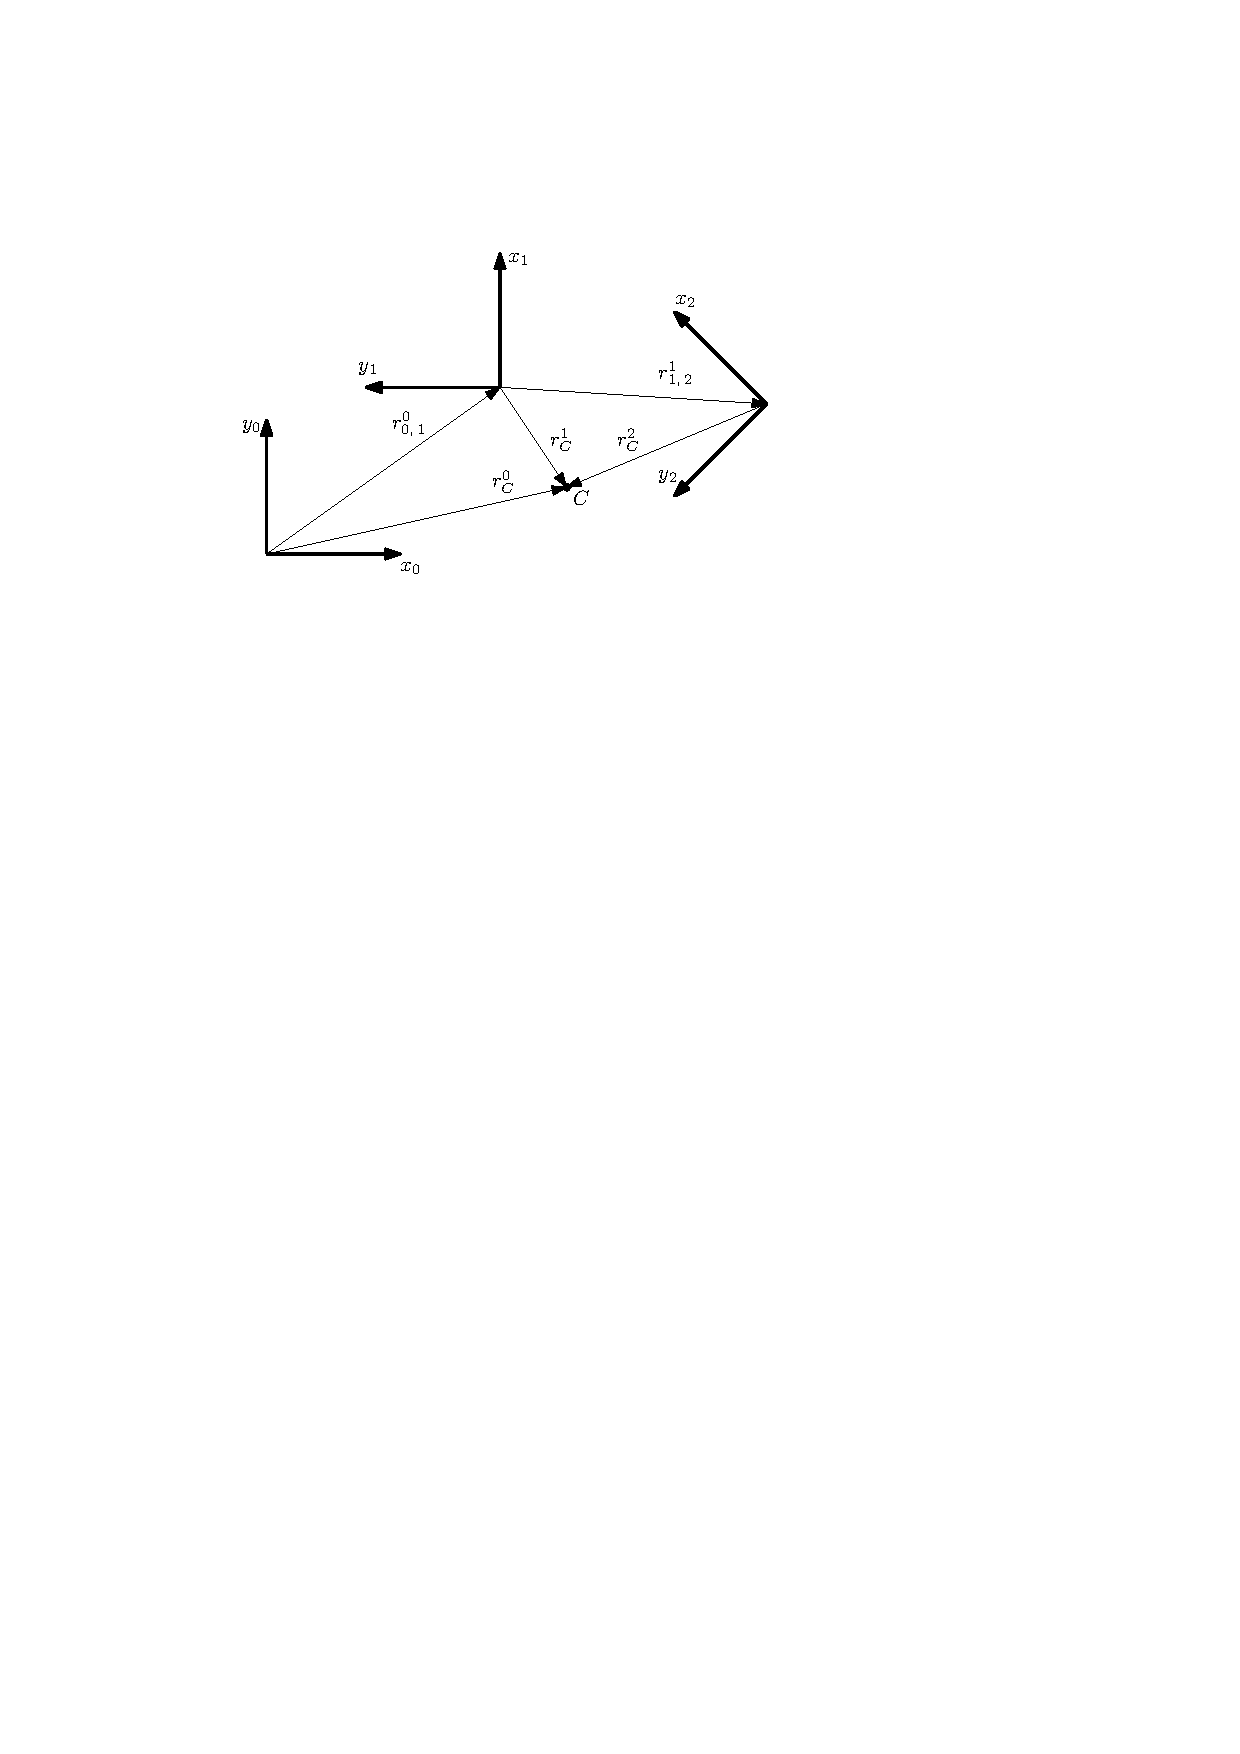
\includegraphics[width=0.7\textwidth]{three_frames.pdf}
	\caption{Системы координат из пояснительного примера.}
	\label{img:three_frames}
\end{figure}